\newpage
\appendix

\section*{Appendix}
\label{sec:appendix}

\section{StyleGAN2 training results}
Displayed in this section are the results of the StyleGAN2 model after training, for reference to the results StylEx achieved.
\begin{figure}[H]
     \centering
     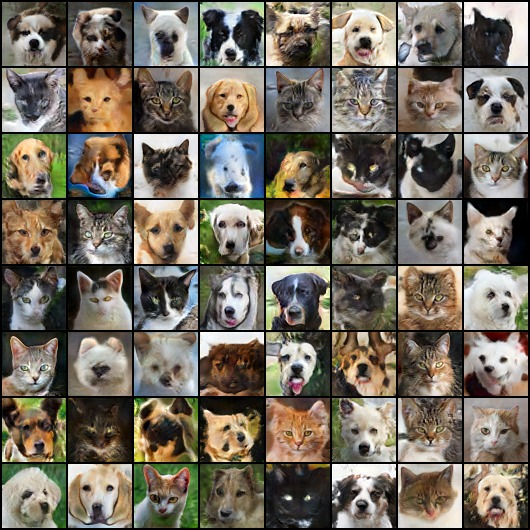
\includegraphics[scale=0.45]{images/Dog_results.jpg}
     \caption{Generated results from the StyleGAN2 on the AFHQ dataset.}
     \label{fig:SG2_Anim}
\end{figure}


\begin{figure}[H]
     \centering
     \includegraphics[scale=0.45]{images/Human_results.jpg}
     \caption{Generated results from the StyleGAN2 on the FFHQ dataset.}
     \label{fig:SG2_Hum}
\end{figure}

\section{Wu \textit{et al.} results}
Below are some results of extracting the most important features of the Wu \textit{et al.} paper.
\begin{figure}[H]
     \centering
     \begin{subfigure}[b]{0.24\textwidth}
     \centering
     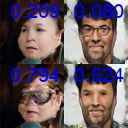
\includegraphics[scale=0.6]{images/Wu_feat1.jpg}
     \caption{Glasses}
     \label{fig:wu1}
     \end{subfigure}
     \hfill
     \begin{subfigure}[b]{0.24\textwidth}
     \centering
     \includegraphics[scale=0.6]{images/Wu_feat2.jpg}
     \caption{Wrinkles}
     \label{fig:wu2}
     \end{subfigure}
     \hfill
     \begin{subfigure}[b]{0.24\textwidth}
     \centering
     \includegraphics[scale=0.6]{images/Wu_feat3.jpg}
     \caption{Eye size}
     \label{fig:wu3}
     \end{subfigure}
     \hfill
     \begin{subfigure}[b]{0.24\textwidth}
     \centering
     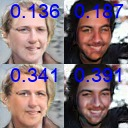
\includegraphics[scale=0.6]{images/Wu_feat4.jpg}
     \caption{Skin tone}
     \label{fig:wu4}
     \end{subfigure}
     \caption{Four most important features found for Wu \textit{et al.}, with the most important feature on the left and the fourth most important feature on the right. Left image at each feature shows the classification score for being classified as old, the right shows the classification score for being classified as young.}
     \label{fig:wu_feats}
\end{figure}

\section{Model architectures}

More detailed architecture of the styleGAN2 model used in the paper.

\begin{figure}[H]
    \centering
    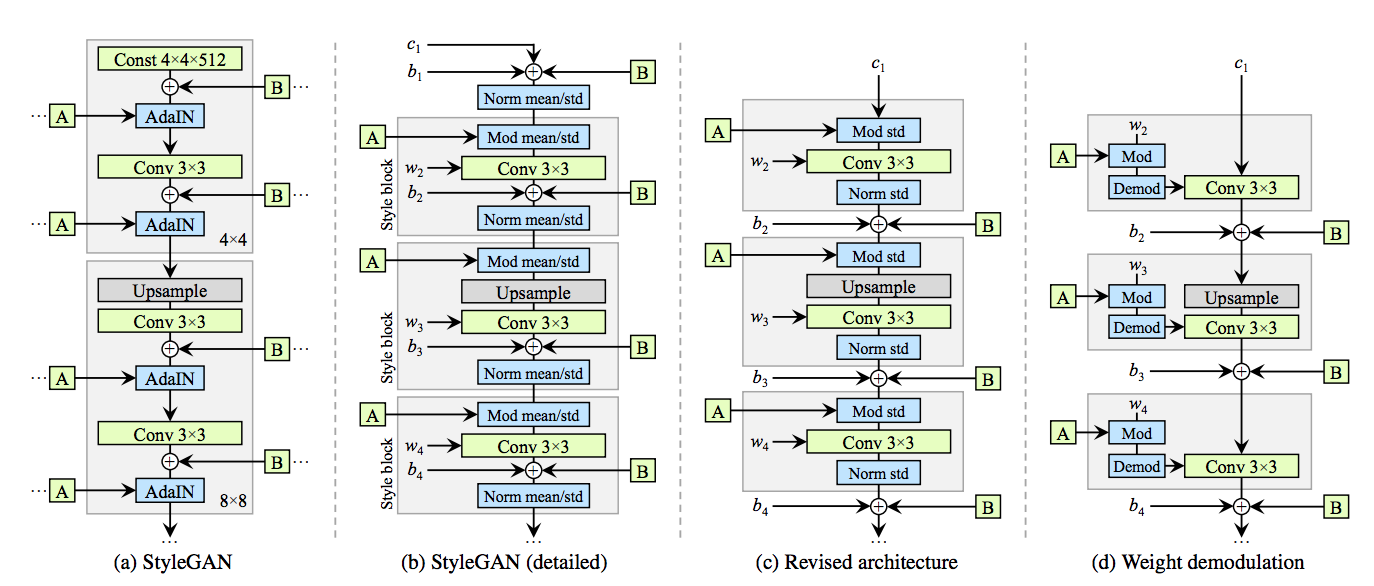
\includegraphics[scale=0.3]{images/StyleGAN2_Arch.png}
    \caption{Original StyleGAN architecture (a and b) alongside the improved StyleGAN2 architecture (c and d), as shown in \cite{karras2020analyzing}. A is a learned affine transform from the latent code and B is some form of noise broadcast operation.}
    \label{fig:StyleGAN2}
\end{figure}

The architecture of the MobileNetV2 model. Used for the classifiers.
\begin{figure}[H]
    \centering
    \includegraphics[scale=0.5]{images/MobileNet.png}
    \caption{MobileNetV2 architecture.}
    \label{fig:MobileV2}
\end{figure}

% \begin{figure}[H]
%      \centering
%      \includegraphics[scale=0.5]{images/AFHQ2.png}
%      \caption{Examples of the AFHQ dataset.}
%      \label{fig:AFHQ}
% \end{figure}

% \begin{figure}[H]
%      \centering
%      \includegraphics[scale=0.5]{images/CelebA.png}
%      \caption{Examples of the CelebA dataset with some associated features.}
%      \label{fig:CelA}
% \end{figure}
